% CS224W Fall 2026 project milestone (project type 1: real-world application of GNNs).
% Compile on Overleaf (upload this folder as a zip) or with: latexmk -pdf milestone.tex
% Every \fillin{...} is a placeholder still to be replaced (it prints in red).

\PassOptionsToPackage{numbers, compress}{natbib}  % numeric citations [1, 2]
\documentclass{article}
\usepackage[final]{neurips_2022}                   % same style file as the proposal
\makeatletter                                      % replace the NeurIPS 2022 footer with the course
\renewcommand{\@noticestring}{CS224W: Machine Learning with Graphs, Stanford University, Fall 2026. Project milestone.}
\makeatother

\usepackage[utf8]{inputenc}
\usepackage[T1]{fontenc}
\usepackage{hyperref}
\usepackage{xurl}                                  % lets long URLs break across lines
\usepackage{booktabs}
\usepackage{amsmath}
\usepackage{amsfonts}
\usepackage{graphicx}
\usepackage{microtype}
\usepackage{dsfont}                                % \mathds{1} for the indicator function
\usepackage{xcolor}
\usepackage{tikz}                                  % Figure 2 (the pipeline)
\usetikzlibrary{arrows.meta, positioning}
\usepackage[font=small, skip=4pt]{caption}
\newcommand{\fillin}[1]{\textcolor{red}{[#1]}}    % placeholder: shows in red until replaced

\title{Worth the Lookup: Budgeted Relational Retrieval\\for Call-List Prioritization}

\author{Max Rodriguez \quad Stanford University \quad \texttt{maxrod@stanford.edu}}

\begin{document}
\maketitle
\vspace{-2em}
\setlength{\abovedisplayskip}{5pt plus 2pt}
\setlength{\belowdisplayskip}{5pt plus 2pt}

\noindent\textbf{Project type:} real-world application of GNNs (blog post + Colab). \textbf{Group:} Max Rodriguez (solo). Not shared with another course.\\
\textbf{Code:} \url{https://github.com/MaxLuisRodriguez/CS224W-fraud-detection-machine-learning-with-graphs/tree/milestone} (the version used for this report, tagged \texttt{milestone}; code map and run commands in the README).

\section{Problem and motivation}

Before each call, a sales rep's AI research agent can look up a prospect's recent activity, the accounts and events it touches, and other buying signals. Every lookup costs something: enrichment credits, LLM tokens, or latency before the dialer connects. No team researches every prospect deeply, so the real decision is \emph{which lookups to make for the whole call list} within a budget. Sales data are linked tables, and the prospects on one list often touch the same accounts and events (Figure~\ref{fig:calllist}). That couples the prospects in two ways.

\emph{Shared information.} Fetching one shared event informs every prospect connected to it, so its value is the sum of its effects on all of them.

\emph{A shared decision.} A rep calls only the top $K$ of the list, so a lookup matters only if it changes who lands in the top $K$, and that depends on everyone else's scores. Suppose five prospects score 0.80, 0.55, 0.53, 0.20 and 0.10, and the rep calls two. A lookup that moves the fourth prospect from 0.20 to 0.30 improves its prediction but changes no call. A lookup that moves the third prospect from 0.53 to 0.60 swaps who gets called.

This separates three goals that are easy to conflate: making each prediction more accurate (cross-entropy), ranking the whole list better (AUROC, average precision), and choosing the right top $K$ (Precision@$K$). Researching prospects one at a time targets none of them for the list as a whole.

\textbf{Research question.} Given a call list of $N$ prospects and a budget of $B$ lookups, which lookups should an agent make so that a graph neural network (GNN) ranks the list best, and in particular picks the right top $K$?

\textbf{Contributions.} The project has three parts so far and a fourth after the milestone. (i)~A relational GNN that scores a prospect when only part of its neighborhood has been retrieved, so a prediction exists at every budget. (ii)~A lookup environment that prices retrieval. It has two actions, \emph{pull} and \emph{enrich}, each costing one unit, and a cache shared across the list, so a shared entity is paid for once. (iii)~A comparison of lookup policies by their \emph{budget frontier}, ranking quality against lookups per prospect, which shows how well each policy allocates a fixed budget. (iv)~After the milestone, a learned policy that predicts each lookup's value for the whole list. The thread running through all four is the gap between three kinds of value: how much a row helps predict (\emph{predictive information}), how much a lookup improves the list's predictions (\emph{retrieval value}), and how much it changes who gets called (\emph{decision value}). The milestone results show these can diverge.

\textbf{Scope after mentor feedback.} Our mentor advised completing the comparison of lookup policies on one dataset before expanding, since learning the lookup value adds significant complexity. Every result below is therefore on \texttt{rel-event}. \texttt{rel-f1} is used only to develop and test code, and \texttt{rel-avito} is a stretch goal. Two hypotheses that compared datasets are re-scoped to one:
\textbf{(H1)} frontiers are concave: with a quarter of a lookup per prospect, a policy recovers most of the AUROC gap between zero lookups and full information;
\textbf{(H2)} a model trained on randomly hidden rows scores higher (AUROC and Precision@13) than one trained on full neighborhoods when little is revealed;
\textbf{(H3, re-scoped)} retrieval value is concentrated: measured as the AUROC gain per lookup when one table is pulled for every prospect, one or two tables account for most of the gain (previously: search results on \texttt{rel-avito});
\textbf{(H4, re-scoped)} the AUROC advantage of a batch-aware policy over a per-prospect policy grows with a list's sharing, defined in Section~\ref{sec:data} (previously: \texttt{rel-event} vs.\ \texttt{rel-avito});
\textbf{(H5)} a learned batch value beats the best heuristic (after the milestone).

\textbf{Status.} Everything below ran on \texttt{rel-event}: the data pipeline, the partially observed GNN, the lookup environment, five policies and the frontier runner. Three findings stand out. With a quarter of a lookup per prospect, the best simple policy recovers 85\% of the AUROC gap between zero lookups and full information (H1). Training on randomly hidden rows makes the model much better when little is revealed (H2). One table, the prospects' own invitation responses, carries nearly all the retrieval value (H3). That explains why researching every prospect a little beats a heuristic that chases shared events, until every prospect has some evidence (H4). One issue is unresolved: a timestamp on the target's own row can postdate the prediction, so comparisons with a strong LightGBM baseline are provisional until we rerun without it (Section~\ref{sec:validity}).

\section{Data and processing}
\label{sec:data}

\begin{figure}[t]
  \centering
  \begin{minipage}[t]{0.47\linewidth}
    \vspace{0pt}
    \centering
    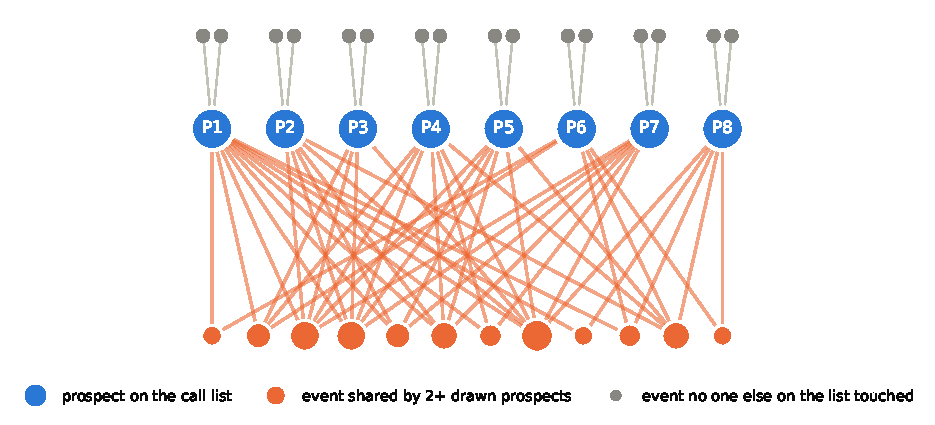
\includegraphics[width=\linewidth]{figures/fig1_call_list.pdf}
    \caption{A real call list (\texttt{rel-event}, 2012-11-21): of a random 128-prospect list, the 8 prospects sharing the most events (blue), their 12 most-shared events (orange; larger = shared by more), and two unshared events each (grey). One orange lookup informs several prospects.}
    \label{fig:calllist}
  \end{minipage}\hfill
  \begin{minipage}[t]{0.49\linewidth}
    \vspace{0pt}
    \centering
    \scriptsize
    \setlength{\tabcolsep}{3pt}
    \begin{tabular}{@{}lrl@{}}
      \toprule
      Table (node type) & Nodes & Foreign keys (edges) \\
      \midrule
      \texttt{users} & 37,143 & -- \\
      \texttt{events} & 2,459,811 & creator (945) \\
      \texttt{event\_attendees} & 8,430,002 & event (8.43M), user (49.8K) \\
      \texttt{event\_interest} & 14,978 & event (14.1K), user (15.0K) \\
      \texttt{user\_friends} & 30,386,403 & user (30.0M), friend (215K) \\
      \bottomrule
    \end{tabular}
    \captionof{table}{The \texttt{rel-event} graph: 41.3M nodes (rows up to the test cutoff), 5 node types, 6 foreign keys giving 12 edge types. An edge exists only where the key points to a row in the database, so most attendance rows link to an event but not to a known user. \texttt{user\_friends} has no timestamp, so friendships are always visible.}
    \label{tab:db}
  \end{minipage}
  \vspace{-0.5em}
\end{figure}

\textbf{Dataset and task.} We use the \texttt{user-ignore} task of \texttt{rel-event} from RelBench~\cite{robinson2024relbench}, a public benchmark of real relational databases with temporal splits. The database comes from an event app (the Kaggle Event Recommendation Engine Challenge; downloaded from Hugging Face, no login needed). Users receive invitations to events and respond yes, maybe or no, or never respond. A prediction is made for a user at a time $t$. The label asks whether the user will ignore more than two invitations in the seven days after $t$, where ignoring means never responding. The label comes from attendance records after $t$; the model sees only records dated at or before $t$. Splits are by time. Training has 19,239 labeled users over 22 prediction dates (16.9\% positive). Validation is one day, 2012-11-21, with 2,013 users (11.1\% positive): a single day's call list, from which we draw lists of 128. The test day (1,958 users) is held out and will be used once, at the end.

\emph{How this stands in for sales.} \texttt{rel-event} is a public stand-in, not sales data. Users play prospects, events play the accounts and events that prospects share, and the label is an engagement outcome to rank a list by. What carries over is the structure our question depends on: linked tables, entities shared across a list, a fixed lookup budget and a top-$K$ decision. We make no claim that the numbers transfer to a CRM.

\textbf{From tables to a graph.} Following relational deep learning (RDL)~\cite{fey2024rdl}, every row becomes a node typed by its table, and every primary--foreign-key link becomes an edge in both directions (\texttt{f2p\_<key>} and its reverse \texttt{rev\_f2p\_<key>}). This gives 5 node types and 12 edge types (Table~\ref{tab:db}). For example, the attendance row (user 17, event 812, status \emph{invited}, dated 2012-11-14) becomes an \texttt{event\_attendees} node with two features, its status and its date, and with edges to user 17 and to event 812 in both directions. RelBench proposes a semantic type for every column. Numerical columns are normalized. Categorical columns get learned embeddings. Text columns, such as a user's location, are embedded with 300-d GloVe word vectors~\cite{pennington2014glove}. RelBench's \texttt{make\_pkey\_fkey\_graph} turns each table into PyTorch Frame tensors; \texttt{events}, for instance, becomes a $2.46\text{M} \times 108$ frame. We cache the result. The first build took 27 minutes and peaked at 30 GB of RAM, and reloading the cache takes about 6 minutes.

\textbf{Time-respecting sampling.} To score a user at time $t$, PyG's temporal \texttt{NeighborLoader}~\cite{fey2019pyg} samples up to 128 neighbors per edge type at hop 1 and 64 at hop 2, only among rows dated at or before $t$. Sampling is disjoint: each target gets its own tree, because two targets can have different prediction times and so may see different parts of the same neighborhood. As a result, an event that two prospects both attended appears twice in a batch, as two separate nodes. The model treats the copies as unrelated, which is fine for prediction. Retrieval must not: an agent that fetches the event once should see it under both prospects. PyG keeps each sampled node's original row id (\texttt{n\_id}), so the two copies share an id, and our lookup cache is keyed on that id (Section~\ref{sec:env}). The time filter applies to sampled neighbors. A target's own row is always included, which matters for one leakage issue (Section~\ref{sec:validity}).

\textbf{Call lists.} A call list is $N = 128$ users drawn at random (seeded) from the validation day. Their neighborhoods are sampled once into one batch, and every policy acts on that same subgraph (Table~\ref{tab:list}). Every prospect has friendship rows, but only 86 of 128 have attendance rows, 15 have interest clicks and 10 created events, so this list offers 239 pulls (1.9 per prospect). We measure a list's \emph{sharing} per entity type as
\begin{equation}
  \text{sharing} = \frac{\left|\{\text{entities listed by two or more prospects}\}\right|}{\left|\{\text{entities listed by any prospect}\}\right|}.
  \label{eq:sharing}
\end{equation}
On this list, 930 distinct events sit behind the attendance rows, and 33\% of them are listed by two or more prospects (our proposal measured 34\%). Of the 1,296 friends who are known users, 11\% are shared. The difference between sampled copies and distinct rows matters for cost: a lookup pays for a distinct row once, however many copies the sampler made. Fetching everything costs 2,752 paid lookups per list on average (2,287--3,509 over 100 lists), about 21.5 per prospect.

\begin{table}[h]
  \centering
  \small
  \begin{tabular}{@{}lrrp{0.5\linewidth}@{}}
    \toprule
    Table & Sampled rows & Distinct & Role in the lookup environment \\
    \midrule
    \texttt{user\_friends} & 17,630 & 17,628 & hop 1 for all 128 prospects (one pull each) \\
    \texttt{event\_attendees} & 1,647 & 1,647 & hop 1 for 86 prospects (1,519 rows); 128 rows of events prospects created \\
    \texttt{event\_interest} & 116 & 116 & hop 1 for 15 prospects \\
    \texttt{events} & 1,672 & 1,060 & hop 2: 930 events behind attendance rows (33\% listed by 2+ prospects); hop 1: 49 created by 10 prospects \\
    \texttt{users} & 1,477 & 1,303 & the 128 prospects, and 1,296 friends who are known users (11\% listed by 2+) \\
    \bottomrule
  \end{tabular}
  \caption{One 128-prospect call list on \texttt{rel-event} (\texttt{scripts/check\_call\_list.py}, list seed 0). Sampled rows count every copy the per-target sampler made; distinct rows count each database row once. One forward pass over the whole list takes 0.41 s on an NVIDIA L4.}
  \label{tab:list}
\end{table}

\section{Model design and metrics}

\begin{figure}[t]
  \centering
  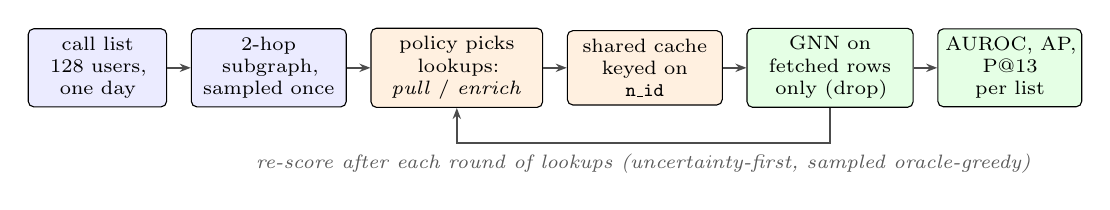
\begin{tikzpicture}[
      box/.style={draw, rounded corners=2pt, align=center, font=\scriptsize, minimum height=2.6em, inner sep=3pt, fill=#1},
      box/.default=white,
      arr/.style={-{Stealth[length=4pt]}, thick, draw=black!70},
      lab/.style={font=\scriptsize\itshape, text=black!65, align=center}]
    \node[box=blue!8, text width=4.4em] (list) {call list\\128 users,\\one day};
    \node[box=blue!8, text width=5.0em, right=0.3cm of list] (sub) {2-hop\\subgraph,\\sampled once};
    \node[box=orange!12, text width=5.6em, right=0.3cm of sub] (pol) {policy picks\\lookups:\\\emph{pull} / \emph{enrich}};
    \node[box=orange!12, text width=5.0em, right=0.3cm of pol] (cache) {shared cache\\keyed on\\\texttt{n\_id}};
    \node[box=green!10, text width=5.4em, right=0.3cm of cache] (gnn) {GNN on\\fetched rows\\only (drop)};
    \node[box=green!10, text width=4.6em, right=0.3cm of gnn] (met) {AUROC, AP,\\P@13\\per list};
    \draw[arr] (list) -- (sub);
    \draw[arr] (sub) -- (pol);
    \draw[arr] (pol) -- (cache);
    \draw[arr] (cache) -- (gnn);
    \draw[arr] (gnn) -- (met);
    \draw[arr] (gnn.south) -- ++(0,-0.45) -| node[lab, pos=0.25, below] {re-score after each round of lookups (uncertainty-first, sampled oracle-greedy)} (pol.south);
  \end{tikzpicture}
  \caption{The evaluation pipeline. A call list is sampled once. A policy spends the budget in rounds of $N/4$ paid lookups; an action whose rows are already cached costs nothing. The trained GNN scores the list from the fetched rows, and the metrics are recorded each time the spend reaches a budget.}
  \label{fig:pipeline}
  \vspace{-0.5em}
\end{figure}

\subsection{Model}
We use RelBench's RDL baseline~\cite{fey2024rdl}, built in PyG~\cite{fey2019pyg}. Each node $v$ has a table type $T(v)$, features $x_v$ (its columns) and a timestamp $\tau(v)$. To score a prospect at time $t$, each row starts as $h_v^{(0)} = \mathrm{Enc}_{T(v)}(x_v) + \phi(t - \tau(v))$: a per-table PyTorch Frame ResNet over its columns, plus an encoding $\phi$ of the row's age at $t$. Two heterogeneous GraphSAGE layers~\cite{hamilton2017sage} then update every node:
\begin{equation}
  h_v^{(\ell+1)} = \mathrm{ReLU}\Big(\mathrm{LN}\Big(\textstyle\sum_{r \in \mathcal{R}(v)} \big[ W^{(\ell)}_{r,1} h_v^{(\ell)} + W^{(\ell)}_{r,2} \sum_{u \in \mathcal{N}_r(v)} h_u^{(\ell)} \big]\Big)\Big).
  \label{eq:sage}
\end{equation}
Here a relation $r$ is a (source type, edge type, target type) triple, and $\mathcal{R}(v)$ holds the relations that end at $v$'s type, for example (\texttt{event\_attendees}, \texttt{f2p\_user\_id}, \texttt{users}). $\mathcal{N}_r(v)$ is the set of $v$'s sampled neighbors under $r$. Each relation has its own weights. $W_{r,2}$ transforms the summed neighbor states and $W_{r,1}$ transforms $v$'s own state, so attendance rows and friendship rows send differently weighted messages. This matches the implementation: PyG's \texttt{SAGEConv} keeps a root weight per relation, and \texttt{HeteroConv} sums across relations. Layer normalization (LN) rescales each node's vector, which keeps the layer stable when a node has very many neighbors. The neighbor states are summed rather than averaged, because a sum keeps counts, such as how many invitations went unanswered, which a mean or a max discards. GIN~\cite{xu2019gin} shows that a sum followed by an MLP is injective on multisets of countable features. Our layer applies a linear map after the sum, so it is not guaranteed to be injective, but it keeps the count information that mean and max remove.

\emph{What two layers compute.} Take a user Ana with two attendance rows: $a_1$ (\emph{invited}, pointing to event $e_1$) and $a_2$ (\emph{yes}, pointing to $e_2$). Layer 1 lets Ana's vector absorb $a_1$ and $a_2$, her response history, and lets $a_1$ and $a_2$ absorb $e_1$ and $e_2$. Layer 2 lets Ana absorb $a_1$ and $a_2$ again, now carrying their events. So two layers reach exactly the two hops our lookups act on: a prospect's own rows, and the entities those rows point to. A linear head with batch normalization maps Ana's final 128-d vector to a logit, and $f_\theta(q)$ is its sigmoid. The model has 5.92M parameters. Training minimizes binary cross-entropy with Adam (learning rate 0.005, batch 512, 20 epochs), as in RelBench.

\subsection{Partial retrieval (our extension)}
The agent sees only $O$, the rows fetched so far; the prospects' own rows are always in $O$. We support two ways to hide the rest (Table~\ref{tab:hide}). In \emph{mask} mode an unfetched row's input is replaced by a learned per-table vector:
\begin{equation}
  \tilde h_v^{(0)} = m_v\, h_v^{(0)} + (1 - m_v)\, e^{\mathrm{mask}}_{T(v)}, \qquad m_v = \mathds{1}[v \in O].
  \label{eq:mask}
\end{equation}
Revelation is keyed on \texttt{n\_id}, so fetching a row reveals all its sampled copies at once. We train two regimes. \emph{Full-trained} uses the standard recipe. \emph{Random-trained} draws a share $p \sim U(0,1)$ per batch and reveals each distinct row with probability $p$, a graph augmentation that shows the model partial views during training. All lookup experiments use drop mode, the mode both regimes were trained in. Mask mode needs its own trained models and is a planned ablation.

\begin{table}[h]
  \centering
  \small
  \begin{tabular}{@{}p{0.27\linewidth}p{0.31\linewidth}p{0.34\linewidth}@{}}
    \toprule
    & Drop & Mask \\
    \midrule
    What the model knows about an unfetched row & Nothing: not its existence, type or edges & That it exists, its table and its edges; its content is a learned placeholder \\
    Effect on a sum in Eq.~\ref{eq:sage} & One fewer term & Same number of terms, placeholder values \\
    Trade-off & Simple; cannot tell ``unread'' from ``absent'' & Keeps structure; needs models trained with placeholders \\
    \bottomrule
  \end{tabular}
  \caption{Two ways to hide rows that have not been fetched. All lookup experiments use drop mode.}
  \label{tab:hide}
\end{table}

\subsection{Lookup environment}
\label{sec:env}
Two actions retrieve rows:
\begin{itemize}
  \setlength\itemsep{0pt}
  \item \texttt{pull}$(i, T)$ reveals all of prospect $i$'s sampled rows in table $T$ (up to 128 per relation). On \texttt{rel-event} these are attendance records, friendships in either direction, interest clicks, or events the user created. A pull also \emph{lists} the entities those rows point to: their ids become known, but their contents do not.
  \item \texttt{enrich}$(T, v)$ reveals exactly one listed row $v$, in every sampled copy: an attended event, a friend who is a known user, or an attendance row of an event the user created.
\end{itemize}
An entity can be enriched only after a pulled row lists it (\emph{list before get}), as with real CRM and enrichment APIs. The accounting is as follows. An action that reveals at least one new row costs one \emph{paid lookup}. An action whose rows are all cached costs nothing, and each pull can be made once. Budgets and costs always count paid lookups, so a budget of $b$ lookups per prospect means $bN$ paid lookups for the list. \emph{Full retrieval} applies every pull and then enriches until nothing new is listed; its paid cost is the list's \emph{full cost}.

\emph{Example.} \texttt{pull}(Ana, attendance) and \texttt{pull}(Ben, attendance) cost one each, and both list event 812. \texttt{enrich}(events, 812) costs one and reveals event 812 under both prospects, so both scores change. A second enrich of 812 would cost nothing.

\textbf{The objective and the batch value.} For a list $Q = \{q_1, \dots, q_N\}$ with labels $y_i$, a policy $\pi$ chooses lookups in sequence. With $O^\pi_B$ its fetched rows after $B$ paid lookups and $M$ a ranking metric, we want $\max_\pi \mathbb{E}\,[M(f_\theta(Q \mid O^\pi_B), y)]$. Ranking metrics are piecewise constant in the scores, so they don't say how much one lookup helped. We therefore score a lookup $a$ by its \emph{batch value}, the list-wide drop in cross-entropy $\ell$:
\begin{equation}
  V(a \mid O) = \textstyle\sum_{i=1}^{N} \big[ \ell\big(f_\theta(q_i \mid O), y_i\big) - \ell\big(f_\theta(q_i \mid O \cup \{a\}), y_i\big) \big].
  \label{eq:value}
\end{equation}
Cross-entropy is a smooth, per-prospect surrogate, and summing it over the list credits a shared entity for every prospect it informs. It measures retrieval value, not decision value: lowering the loss of a prospect far from the cutoff raises $V$ without changing who gets called. Section~\ref{sec:e3} shows that this matters. $V$ needs labels, so for now we use it only in a reference policy; after the milestone a second model will learn to predict it (H5).

\subsection{Policies}
Every policy proposes the next lookups for the whole list in rounds of $N/4 = 32$ paid lookups. None of the five is learned.
\textbf{Random} picks uniformly among legal lookups; it is the floor.
\textbf{Case-local} lets the least-researched prospect take its own next lookup: its next table, then the entity its rows mention most. Tables are taken in alphabetical order, which on \texttt{rel-event} puts \texttt{event\_attendees} first; Section~\ref{sec:e4} shows that this ordering matters.
\textbf{Uncertainty-first} does the same with prospects ordered by $p(1-p)$, re-scored each round, as in per-instance active feature acquisition~\cite{norcliffe2025sefa,valancius2024aco}.
\textbf{Coverage} is batch-aware: it takes the lookups that inform the most prospects first. A listed entity informs every prospect whose pulled rows point to it; a pull informs one.
\textbf{Sampled oracle-greedy} is a label-informed reference. Each round it samples 64 legal lookups, computes their true $V$ with the labels, and takes the best. It is not deployable, and it is not a guaranteed upper bound: it sees only 64 candidates per round and plans greedily.

\subsection{Metrics}
E1 reports RelBench's official validation AUROC on all 2,013 validation users, as mean $\pm$ s.d.\ over three seeds. Lookup experiments report, per call list, AUROC, average precision (AP) and Precision@$K$: the share of true positives among the $K = \lceil 0.1N \rceil = 13$ highest-scored prospects. A random ranking scores the positive rate, about 0.11. We average over lists and give 95\% percentile-bootstrap intervals over lists (2,000 resamples). Lists, not prospects, are the units, because prospects on one list share entities. Every policy runs on the same lists and subgraphs in one run, so comparisons are paired. Two limitations apply. The intervals cover list-to-list variation for one trained model on one day, not training-seed variation. And lists are drawn from the same 2,013 users, so each user appears on about six of 100 lists; the lists are not fully independent, and the intervals are likely somewhat narrow.

\section{Results so far}
All numbers are on the \texttt{rel-event} validation day (2012-11-21) unless marked; \texttt{rel-f1} is the development dataset. Runs: one NVIDIA L4 GPU on AWS, Nov 7--8.

\subsection{Validity checks}
\label{sec:validity}
\textbf{Implementation.} Eleven unit tests pass on the laptop and the GPU machine. They cover the per-list metrics, temporal sampling, the environment's guarantees (full retrieval equals the full model, cache hits are free, list before get), and that every policy spends exactly its budget in paid lookups using legal actions. On both datasets, \texttt{check\_reveal.py} found that random revelation never splits the copies of a shared row, and that with every row revealed both drop and mask mode reproduce the full model exactly. \texttt{check\_lookup.py} confirmed on both datasets that zero lookups reproduce the model's $p = 0$ scores and full retrieval reproduces its full-information scores. On one \texttt{rel-event} list, full retrieval took 2,555 paid lookups and revealed every sampled row.

\textbf{Temporal leakage.} \texttt{check\_leakage.py} found no sampled neighbor dated after its target's prediction time: none among 431,731 timestamped rows on \texttt{rel-f1}, and none among 145,217 on \texttt{rel-event} (all four timestamped tables, 5 training and 5 validation batches). It did flag target rows. RelBench's task table includes users before their recorded \texttt{joinedAt}: 35\% of training targets and 52 of 2,013 validation targets. A target's own row is always in its subgraph, so every model sees that \texttt{joinedAt}, LightGBM and RelBench's baselines included, and it leaks a little: those 52 validation users are 17\% positive against 11\% overall. All comparisons with LightGBM are therefore provisional until we rerun without \texttt{joinedAt}, and the GNN numbers may shift slightly too.

\textbf{Why attendance history is not the label.} Attendance rows are dated by their event's start time. A prediction at $t$ therefore sees only invitations to events that had started by $t$, while the label concerns invitations in the week after $t$, whose rows are never sampled. One assumption remains: a row's status is the database's final snapshot, so a response given after $t$ to an earlier invitation would be visible. RelBench makes the same assumption. We expect such late responses to be rare, but we have not measured how rare.

\subsection{Training on partial views, and the decision gate (E1, E2)}
Table~\ref{tab:e1} reports validation AUROC when each distinct sampled row is revealed with probability $p$. The full-trained GNN scores $0.818 \pm 0.030$ with every row and $0.612 \pm 0.046$ with none. The random-trained model has a higher mean at every $p$, and the difference is largest when little is revealed: 0.136 at $p = 0$ (0.748 vs.\ 0.612) and 0.062 at $p = \frac14$. With three seeds per regime, the first difference is well beyond the seed spread (Welch $t \approx 4.9$) and the second is suggestive ($t \approx 2.3$). At $p \geq \frac12$ the differences are within seed variation. Precision@13 tells the same story. From $p = 1$ to $p = 0$, the full-trained model drops from 0.563 to 0.166 and the random-trained model from 0.574 to 0.265.

\begin{table}[h]
  \centering
  \small
  \setlength{\tabcolsep}{3.5pt}
  \begin{tabular}{@{}llccccc@{}}
    \toprule
    Dataset & Training & $p = 1$ & $p = 0.75$ & $p = 0.5$ & $p = 0.25$ & $p = 0$ \\
    \midrule
    \texttt{rel-event} & full & $0.818 \pm 0.030$ & $0.818 \pm 0.035$ & $0.815 \pm 0.039$ & $0.794 \pm 0.045$ & $0.612 \pm 0.046$ \\
    \texttt{rel-event} & random & $0.853 \pm 0.020$ & $0.859 \pm 0.017$ & $0.862 \pm 0.015$ & $0.856 \pm 0.013$ & $0.748 \pm 0.015$ \\
    \texttt{rel-f1} (dev) & full & $0.773 \pm 0.027$ & $0.778 \pm 0.027$ & $0.772 \pm 0.028$ & $0.763 \pm 0.025$ & $0.655 \pm 0.031$ \\
    \midrule
    \multicolumn{7}{@{}l}{LightGBM on the prospect's own row only (provisional; see Section~\ref{sec:validity}): \texttt{rel-event} 0.853, \texttt{rel-f1} 0.661} \\
    \bottomrule
  \end{tabular}
  \caption{Validation AUROC on all validation targets, mean $\pm$ s.d.\ over 3 training seeds, when each distinct sampled row is revealed with probability $p$ (hidden rows dropped). Full: standard training. Random: a share $p \sim U(0,1)$ revealed per training batch.}
  \label{tab:e1}
\end{table}

\emph{Why training on partial views helps.} The likely mechanism is a match between training and inference. A full-trained model only ever saw complete neighborhoods, so when most rows are hidden its inputs look unlike anything it was trained on. A random-trained model has seen near-empty and half-empty neighborhoods, and it learned to rely on whatever is present, including the prospect's own row. This reverses our \texttt{rel-f1} result from the proposal, and we do not yet know why. \texttt{rel-f1} has far fewer training targets (1,353 vs.\ 19,239) and a different neighborhood structure, and either could matter, but we have not tested them.

\textbf{A strong but provisional baseline.} LightGBM on the prospect's own row (locale, birthyear, gender, joinedAt, location, timezone) reaches 0.853 validation AUROC. That equals the random-trained GNN with every row and beats the full-trained GNN. On call lists it scores AP 0.568 and Precision@13 0.545, slightly below the full-information GNN (about 0.58--0.60 and 0.56--0.57). Two readings are possible. Profile features may carry much of the AUROC signal on this day, with boosted trees using them better than the GNN's row encoder. Or the \texttt{joinedAt} leak may help the trees more than the GNN. The rerun without \texttt{joinedAt} will separate the two, and it will also show how much of the GNN's own signal comes from attendance histories. Until then we treat LightGBM as a reference line, not a benchmark. The leaderboard's test numbers in our proposal (GNN 0.804, LightGBM 0.773) come from a different day and are not comparable.

\textbf{E2: the decision gate.} A lookup policy moves a list somewhere between zero lookups and full information, so that gap bounds what any policy can show. If it were tiny, every policy would look the same. Before running frontiers we agreed with our mentor to proceed only if $\Delta = \text{AUROC}(p{=}1) - \text{AUROC}(p{=}0) \geq 0.02$ for the full-trained model. Seed-to-seed spread on \texttt{rel-f1} was 0.02--0.05, so a smaller gap could not separate policies. On \texttt{rel-event}, $\Delta = 0.818 - 0.612 = 0.206$, so \texttt{rel-event} remains the dataset of record and \texttt{rel-avito} a stretch goal.

\subsection{Budget frontiers (E3)}
\label{sec:e3}
Figure~\ref{fig:frontier} runs all five policies on the same 100 call lists, at budgets from $\frac14$ to 16 paid lookups per prospect. The lists are scored by the seed-0 full-trained model, chosen before any frontier ran. We summarize a policy at budget $b$ by the share of the gap it recovers,
\begin{equation}
  \text{gap recovered}(b) = \frac{M_{\text{policy}}(b) - M_{\text{zero}}}{M_{\text{full}} - M_{\text{zero}}},
  \label{eq:gap}
\end{equation}
where $M_{\text{zero}}$ is a list's score with only the prospects' own rows and $M_{\text{full}}$ its score after full retrieval.

\textbf{H1: concave frontiers.} With 32 paid lookups for 128 prospects ($b = \frac14$, about 1.2\% of the cost of full retrieval), case-local reaches 0.752 AUROC per list, against 0.597 with zero lookups and 0.780 with full information. That is $(0.752 - 0.597)/(0.780 - 0.597) = 85\%$ of the gap. An earlier, independently sampled run on 30 lists gave 81\%. From $b = \frac12$, case-local exceeds full information (0.802 vs.\ 0.780). On Precision@13 it reaches 0.542 at $b = 1$, against 0.549 with everything fetched. At $b = 16$, every heuristic except random is within 0.003 of full information. That is expected: at large budgets all policies have revealed nearly the same rows.

These zero and full values differ from E1's (0.612 and 0.818) for two reasons. E3 uses only the seed-0 model, the weakest of the three (0.784 on the full validation set). And it averages AUROC within 128-prospect lists instead of computing it once over all 2,013 users.

\textbf{The policies differ by more than their intervals.} Paired with case-local on the same lists at $b = 1$, coverage is $-0.097$ AUROC (95\% interval $[-0.114, -0.078]$), uncertainty-first $-0.105$ $[-0.119, -0.091]$ and random $-0.169$ $[-0.192, -0.148]$. Sampled oracle-greedy is $+0.069$ $[0.055, 0.084]$.

\textbf{Why coverage loses early and wins later.} Coverage maximizes \emph{entity-level coverage}: how many prospects each lookup informs. A ranking also needs \emph{prospect-level coverage}: how many prospects have any evidence at all. The two pull in different directions. In its first round, coverage has nothing listed yet, so it pulls 32 prospects. From then on, any event shared by two of those 32 informs two prospects, so it outranks every remaining pull, which informs one. By $b = 1$, coverage has made 87 event enrichments and only 16 attendance pulls, and most prospects have no evidence. We call this \emph{starvation}. Case-local does the opposite. Its first lookup for almost every prospect is the attendance table: 28.9 of its first 32 lookups, and by $b = 1$ all of the roughly 90 prospects that have attendance rows. Uncertainty-first starves in a milder way, returning to the same uncertain prospects. Once every prospect has evidence, shared entities become the better buy: at $b = 4$ and $b = 8$, coverage edges ahead of case-local ($+0.010$ $[0.001, 0.019]$ and $+0.013$ $[0.009, 0.016]$). Together these results suggest a two-stage strategy: first give every prospect a minimum of evidence, then spend on shared entities. That is the breadth-then-share heuristic we test next (Section~\ref{sec:next}).

\textbf{Retrieval value is not decision value.} Sampled oracle-greedy picks lookups by their true $V$. It gains $+0.069$ AUROC over case-local at $b = 1$ but loses on Precision@13 (0.490 vs.\ 0.542). Lowering the list's cross-entropy improves the ranking overall, but it does not necessarily put the right prospects in the top 13. This is direct evidence that the surrogate in Eq.~\ref{eq:value} and the decision a rep makes can diverge, and it motivates a cutoff-aware value for H5.

\begin{figure}[t]
  \centering
  \begin{minipage}[t]{0.495\linewidth}
    \centering
    \IfFileExists{figures/frontier_rel-event_auroc.pdf}{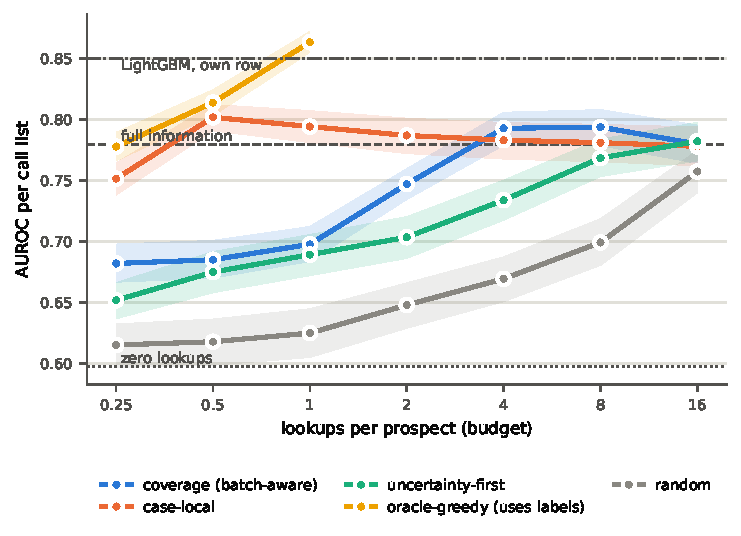
\includegraphics[width=\linewidth]{figures/frontier_rel-event_auroc.pdf}}{\fbox{AUROC frontier}}\\[-2pt]
    {\footnotesize (a) AUROC per call list}
  \end{minipage}\hfill
  \begin{minipage}[t]{0.495\linewidth}
    \centering
    \IfFileExists{figures/frontier_rel-event_p_at_k.pdf}{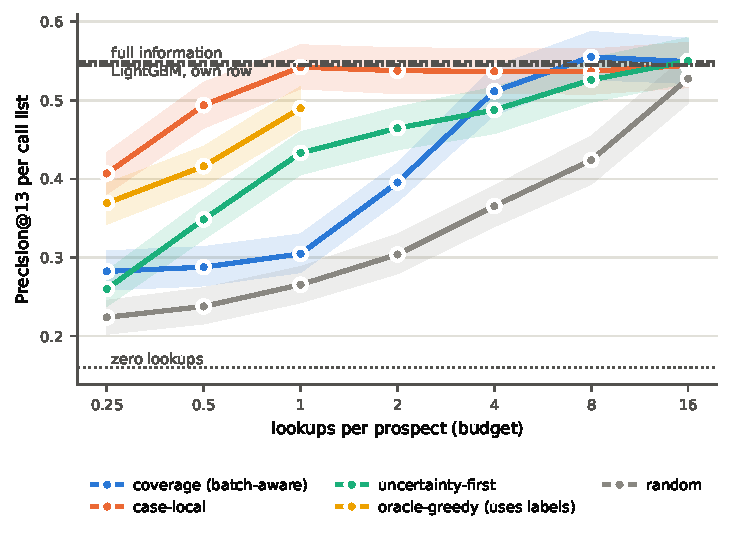
\includegraphics[width=\linewidth]{figures/frontier_rel-event_p_at_k.pdf}}{\fbox{P@13 frontier}}\\[-2pt]
    {\footnotesize (b) Precision@13 per call list}
  \end{minipage}
  \caption{Budget frontiers on \texttt{rel-event}: mean metric per 128-prospect call list against paid lookups per prospect (log scale), 100 lists, seed-0 full-trained model; bands are 95\% bootstrap intervals over lists. Dotted: zero lookups. Dashed: full information (on average 2,752 paid lookups per list). Dash-dot: LightGBM on the prospect's own row, provisional (Section~\ref{sec:validity}), scored on 200 random lists of the same day. Oracle-greedy is the sampled, label-informed reference policy and is run only to $b = 1$.}
  \label{fig:frontier}
\end{figure}

\begin{figure}[t]
  \centering
  \IfFileExists{figures/frontier_rel-event_auroc_random_trained.pdf}{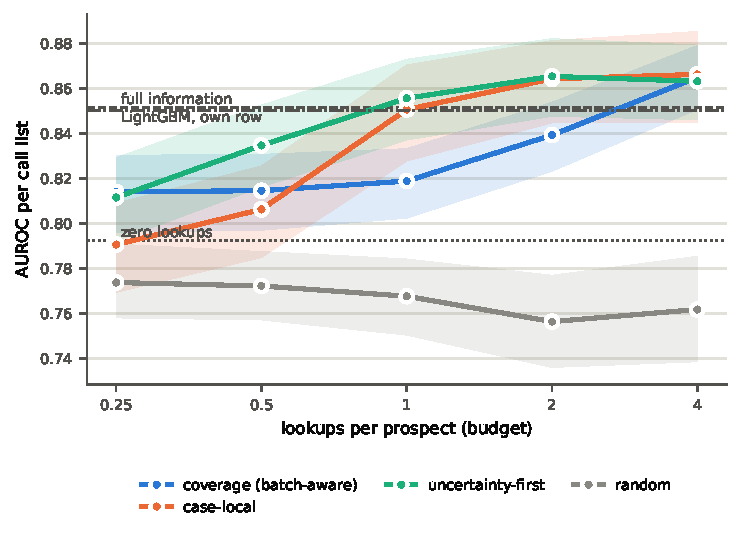
\includegraphics[width=0.62\linewidth]{figures/frontier_rel-event_auroc_random_trained.pdf}}{\fbox{random-trained frontier}}
  \caption{The AUROC frontier with the random-trained model (seed 0): 30 call lists, four policies, 95\% bootstrap bands. Dotted: zero lookups (0.792). Dashed: full information (0.852). Dash-dot: LightGBM on the prospect's own row (0.850, provisional). A separate run from Figure~\ref{fig:frontier}, so the two are not paired list by list.}
  \label{fig:random}
\end{figure}

\textbf{H2 under chosen lookups.} Figure~\ref{fig:random} repeats the frontier with the seed-0 random-trained model on 30 lists. This is a separate run, so it is not paired with Figure~\ref{fig:frontier}. The random-trained model starts much higher with zero lookups, 0.792 against 0.597. With case-local it reaches 0.866 at $b = 4$, above its own full information (0.852) and above the provisional LightGBM reference (0.850). With this model, the policy order changes at small budgets. Uncertainty-first and coverage beat case-local at $b = \frac14$ (paired $+0.021$ $[0.004, 0.037]$ and $+0.023$ $[0.016, 0.031]$), and uncertainty-first also leads on Precision@13 (0.456 vs.\ 0.387). Case-local catches up once every prospect's attendance has been pulled ($b = 1$: 0.851). Under these conditions, the model's uncertainty became a useful guide only when the model had been trained on partial views.

\subsection{What is worth a lookup (E4)}
\label{sec:e4}
Table~\ref{tab:value} pulls one table for every prospect, then enriches everything those rows list, and measures the AUROC gain over zero lookups. Under the current model and training regime, one table carries the retrieval value. Pulling attendance histories (89 paid lookups per list) raises AUROC by 0.224 $[0.188, 0.261]$, and enriching the roughly 1,000 events they list adds only 0.002 more. Interest clicks change nothing. Pulling the events a prospect created lowers AUROC by 0.029, and pulling friendships lowers it by 0.062, both with intervals that exclude zero.

Attendance rows hold each past invitation's response (invited, yes, maybe, no), the most direct evidence of whether a user answers invitations. Section~\ref{sec:validity} explains why they do not reveal the future label. The negative values are not evidence that friendships carry no signal. They show that this model, trained with every row present, does not use friendship and created-event rows well on this day. The extra rows may add noise, or 128 featureless friendship rows may swamp the summed message at layer 2; separating these needs the ablations in Section~\ref{sec:next}.

This also explains two earlier observations. Case-local leads at small budgets because its first lookup per prospect is the valuable one, and partial retrieval can beat full retrieval because full retrieval adds rows that this model handles poorly. Case-local reaches attendance first because it takes a prospect's tables in alphabetical order, and \texttt{event\_attendees} sorts first. Its result therefore reflects an interaction between lookup order and where the value sits across tables. A case-local with a value-aware table order is the fair version to compare against.

\begin{table}[h]
  \centering
  \small
  \begin{tabular}{@{}lrrrrr@{}}
    \toprule
    Table pulled for every prospect & \multicolumn{3}{c}{Pull only} & \multicolumn{2}{c}{Pull + enrich} \\
    \cmidrule(lr){2-4}\cmidrule(l){5-6}
    & lookups & AUROC gain [95\% interval] & per 100 & lookups & gain \\
    \midrule
    \texttt{event\_attendees} & 89 & $+0.224$ $[+0.188, +0.261]$ & $+0.251$ & 1,122 & $+0.226$ \\
    \texttt{event\_interest} & 11 & $+0.000$ $[-0.018, +0.019]$ & $+0.004$ & 93 & $+0.002$ \\
    \texttt{events} (created) & 7 & $-0.029$ $[-0.046, -0.014]$ & $-0.395$ & 183 & $-0.033$ \\
    \texttt{user\_friends} & 128 & $-0.062$ $[-0.107, -0.016]$ & $-0.048$ & 1,447 & $-0.089$ \\
    \bottomrule
  \end{tabular}
  \caption{Value of each table: AUROC gain over zero lookups when one table is pulled for every prospect (and, right, when everything those rows list is enriched too), mean over 30 call lists, seed-0 full-trained model (\texttt{scripts/table\_value.py}). ``Per 100'': gain per 100 paid lookups. A first run on 10 lists gave the same signs for attendance, created events and friendships.}
  \label{tab:value}
\end{table}

\subsection{Sharing and batch-awareness (E5)}
We split the 100 lists into thirds by sharing (Eq.~\ref{eq:sharing}, over all entity types) and compare coverage with case-local, averaging the paired AUROC difference over $b \leq 2$. Coverage's deficit grows with sharing: $-0.067$ $[-0.087, -0.049]$ on the least-shared third (11--16\% shared), $-0.076$ $[-0.097, -0.056]$ on the middle third (16--19\%), and $-0.099$ $[-0.118, -0.080]$ on the most-shared third (19--24\%). The paired strata are the main evidence; the per-list correlation between sharing and coverage's advantage is weak ($-0.17$). The mechanism matches E3. On lists that share more, more of coverage's budget goes to events shared among the prospects it pulled first, and more prospects are left without evidence. At small budgets, then, this heuristic contradicts H4. That is a finding about coverage's starvation, not about batch-aware retrieval in general. The test is also limited: sharing ranges only from 11\% to 24\% across random lists of one day.

\textbf{Summary against the hypotheses.} H1: supported (85\% of the gap at about 1\% of the cost, replicated on a separate 30-list run). H2: supported under random revelation when little is revealed, and under chosen lookups (the random-trained frontier starts at 0.792 and reaches 0.866). H3 (re-scoped): supported for this model (attendance histories carry the retrieval value; friendships and created events lower AUROC). H4 (re-scoped): not supported at small budgets by the one batch-aware heuristic tested, which starves prospects, and more so on lists that share more; a small batch-aware advantage appears at $b \geq 4$. H5: next.

\section{Next steps}
\label{sec:next}
The results change what the learned policy must do. It has to cover every prospect first, know which table is worth a lookup, and value moving prospects across the call cutoff rather than only lowering loss. Table~\ref{tab:next} orders the remaining work by priority.

\begin{table}[h]
  \centering
  \small
  \begin{tabular}{@{}rp{0.36\linewidth}p{0.38\linewidth}l@{}}
    \toprule
    & Experiment & Why & When \\
    \midrule
    1 & Remove \texttt{joinedAt}; rerun E1, LightGBM and the main frontier & Establish validity & Nov 12--18 \\
    2 & Breadth-then-share heuristic & Fixes starvation; tests the two-stage strategy & Nov 12--18 \\
    3 & Case-local with value-aware and randomized table order & Tests whether lookup order explains its lead & Nov 12--18 \\
    4 & Learned, cutoff-aware lookup value (H5) & Aligns the policy with the top-13 decision & Nov 19--30 \\
    5 & Full- vs.\ random-trained frontiers, paired, more seeds & Isolates the effect of partial-view training & Nov 19--30 \\
    6 & Mask vs.\ drop mode & Tests representing unfetched rows & Nov 19--30 \\
    7 & Mean aggregation, GAT~\cite{velickovic2018gat}, LightGBM score as a GNN input & Do the findings depend on the GNN? & late Nov \\
    8 & Larger lists ($N \in \{32, 128, 512\}$), test day, \texttt{rel-avito} & External validity & Dec \\
    \bottomrule
  \end{tabular}
  \caption{Remaining work, in priority order.}
  \label{tab:next}
\end{table}

\textbf{The learned policy (H5).} E3's oracle result is the motivation: a value that only lowers loss does not target the decision. On training-day call lists, where labels are available, we will run the existing policies to reach a variety of states, then compute the true $V$ of sampled candidate lookups. We will also compute a cutoff-aware variant that weights each prospect's loss change by its closeness to the top-13 boundary. We then train a model to predict these values without labels: first from hand-built features of the lookup and the prospects it touches, then with a GNN on the revealed graph, using a list-level head and a singleton head as in per-node query valuation~\cite{zhou2026scout}. At test time the policy takes the highest-valued lookup, re-scores and repeats, in the same frontier runner as the heuristics.

\textbf{Deliverables (to Dec 10).} A Colab that rebuilds the graph, trains the model and draws the frontiers on a small budget, and a Medium post built around Figures~\ref{fig:calllist} and~\ref{fig:frontier}.

\small
\bibliographystyle{plainnat}
\bibliography{refs}

\end{document}
